%
%===============>>  Симонов Модуль 6 <<=============
%=
\setmodule{6}

%BEGIN_FOLD % ====>>_____ Занятие 1 _____<<====
\begin{class}[number=1]
	\begin{listofex}
		\item В таблице даны размеры (с точностью до мм) четырёх листов, имеющих форматы \( A0 \), \( A1 \), \( A3 \), \( A4 \).
		\begin{center}
			\footnotesize
			\begin{tabular}{|c|c|c|}
				\hline
				\rowcolor{gray}\textbf{Номер листа}&\textbf{Длина(мм)}&\textbf{Ширина мм}\\
				\hline
				\( 1 \)&\( 297 \)&\( 210 \)\\
				\hline
				\( 2 \)&\( 420 \)&\( 297 \)\\
				\hline
				\( 3 \)&\( 1189 \)&\( 841 \)\\
				\hline
				\( 4 \)&\( 841 \)&\( 594 \)\\
				\hline
			\end{tabular}
		\end{center}
		Установите соответствие между форматами и номерами листов. В ответ запишите последовательность четырёх цифр, соответствующих номерам листов, без пробелов, запятых и дополнительных символов.
		\begin{center}
			\footnotesize
			\begin{tabular}{|c|c|c|c|}
				\hline
				\textbf{\( A0 \)}&\textbf{\( A1 \)}&\textbf{\( A3 \)}&\textbf{\( A4 \)}\\
				\hline
				\(  \)&\(  \)&\(  \)&\(  \)\\
				\hline
			\end{tabular}
		\end{center}
		Общепринятые форматы листов бумаги обозначают буквой \( A \) и цифрой: \( A0 \), \( A1 \), \( A2 \) и так далее. Лист формата \( A0 \) имеет форму прямоугольника, площадь которого равна \( 1 \) кв. м. Если лист формата А0 разрезать пополам параллельно меньшей стороне, получается два равных листа формата \( A1 \). Если лист \( A1 \) разрезать так же пополам, получается два листа формата \( A2 \). И так далее.
		\begin{center}
			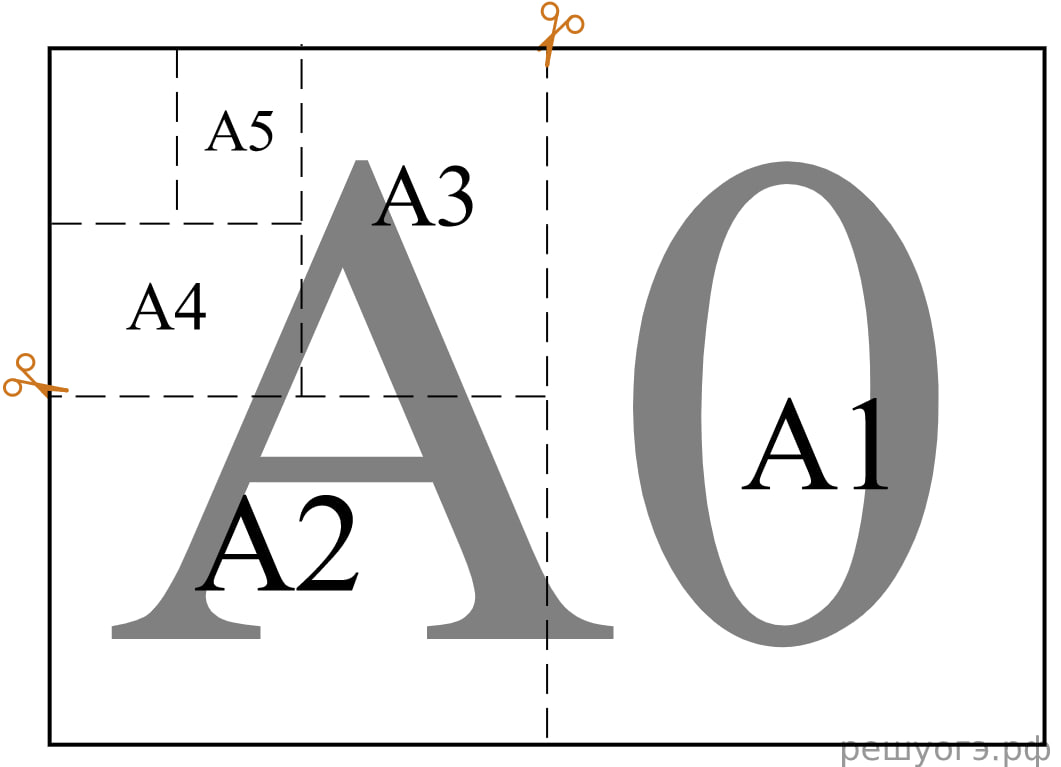
\includegraphics[align=t, width=0.4\linewidth]{../../pics/G91M6L1}
		\end{center}
		Отношение большей стороны к меньшей стороне листа каждого формата одно и то же, поэтому листы всех форматов подобны. Это сделано специально для того, чтобы пропорции текста и его расположение на листе сохранялись при уменьшении или увеличении шрифта при изменении формата листа.
		\item Сколько листов формата \( A3 \) получится из одного листа формата \( A2 \)?
		\item Найдите площадь листа формата \( A1 \). Ответ дайте в квадратных сантиметрах.
		\item Найдите отношение длины меньшей стороны листа формата \( A3 \) к большей. Ответ округлите до десятых.
		\item Бумагу формата \( A5 \) упаковали в пачки по \( 500 \) листов. Найдите массу пачки, если масса бумаги площади \( 1 \) кв. м равна \( 80 \) г. Ответ дайте в граммах.
			\item Решите уравнения:
		\begin{tasks}(2)
			\task \( 2x^2+x=0 \)
			\task \( -3x^2-12x=0 \)
			\task \( 7x^2+14x=0 \)
			\task \( 8x^2+3x=0 \)
			\task \( x^2=64 \)
			\task \( x^2=36 \)
			\task \( -x^2+25=0 \)
			\task \( 100-x^2=0 \)
			\task \( x^2-8x+12=0 \)
			\task \( 15-2x-x^2=0 \)
			\task \( x^2-4x+3=0 \)
			\task \( x^2-4x+4=0 \)
			\task \( 10x^2-17x+34=7x^2-26x+28 \)
			\task \( (x-6)^2=-24x \)
			\task \( x^2+9=(x+9)^2 \)
			\task \( (2x+7)^2=(2x-1)^2 \)
		\end{tasks}
	\end{listofex}
\end{class}
%END_FOLD

%BEGIN_FOLD % ====>>_ Домашняя работа 1 _<<====
\begin{homework}[number=1]
	\begin{listofex}
		\item В таблице даны размеры (с точностью до мм) четырёх листов, имеющих форматы \( A0 \), \( A1 \), \( A3 \), \( A4 \).
		\begin{center}
			\footnotesize
			\begin{tabular}{|c|c|c|}
				\hline
				\rowcolor{gray}\textbf{Номер листа}&\textbf{Длина(мм)}&\textbf{Ширина мм}\\
				\hline
				\( 1 \)&\( 297 \)&\( 210 \)\\
				\hline
				\( 2 \)&\( 420 \)&\( 297 \)\\
				\hline
				\( 3 \)&\( 1189 \)&\( 841 \)\\
				\hline
				\( 4 \)&\( 841 \)&\( 594 \)\\
				\hline
			\end{tabular}
		\end{center}
		Установите соответствие между форматами и номерами листов. В ответ запишите последовательность четырёх цифр, соответствующих номерам листов, без пробелов, запятых и дополнительных символов.
		\begin{center}
			\footnotesize
			\begin{tabular}{|c|c|c|c|}
				\hline
				\textbf{\( A0 \)}&\textbf{\( A1 \)}&\textbf{\( A3 \)}&\textbf{\( A4 \)}\\
				\hline
				\(  \)&\(  \)&\(  \)&\(  \)\\
				\hline
			\end{tabular}
		\end{center}
		Общепринятые форматы листов бумаги обозначают буквой \( A \) и цифрой: \( A0 \), \( A1 \), \( A2 \) и так далее. Лист формата \( A0 \) имеет форму прямоугольника, площадь которого равна \( 1 \) кв. м. Если лист формата А0 разрезать пополам параллельно меньшей стороне, получается два равных листа формата \( A1 \). Если лист \( A1 \) разрезать так же пополам, получается два листа формата \( A2 \). И так далее.
		\begin{center}
			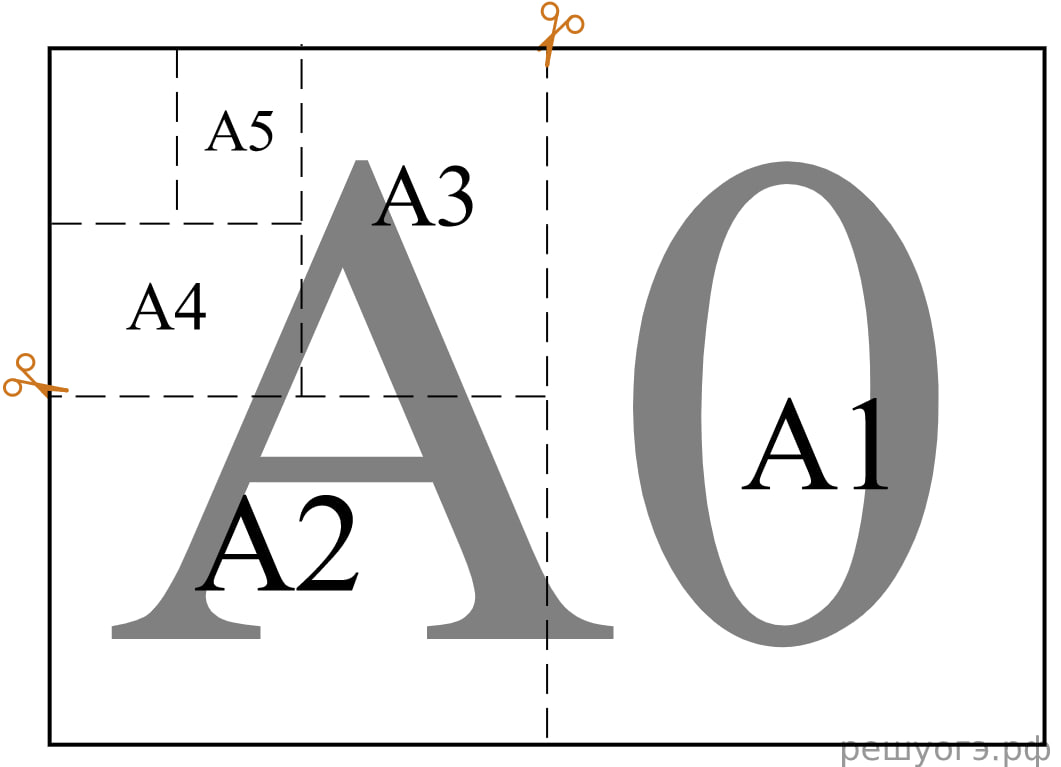
\includegraphics[align=t, width=0.4\linewidth]{../../pics/G91M6L1}
		\end{center}
		Отношение большей стороны к меньшей стороне листа каждого формата одно и то же, поэтому листы всех форматов подобны. Это сделано специально для того, чтобы пропорции текста и его расположение на листе сохранялись при уменьшении или увеличении шрифта при изменении формата листа.
		\item Сколько листов формата \( A5 \) получится из одного листа формата \( A1 \)?
		\item Найдите площадь листа формата \( A6 \). Ответ дайте в квадратных сантиметрах.
		\item Найдите отношение длины большей стороны листа формата \( A2 \) к меньшей. Ответ округлите до десятых.
		\item Бумагу формата \( A3 \) упаковали в пачки по \( 250 \) листов. Найдите массу пачки, если масса бумаги площади \( 1 \) кв. м равна \( 120 \) г. Ответ дайте в граммах.
		\item Решите уравнения:
		\begin{tasks}(2)
			\task \( 2x^2-10x=0 \)
			\task \( x^2+3x=4 \)
			\task \( (x-4)^2+(x+9)^2=2x^2 \)
			\task \( (x+10)^2=(5-x)^2 \)
		\end{tasks}
	\end{listofex}
\end{homework}
%END_FOLD

%BEGIN_FOLD % ====>>_____ Занятие 2 _____<<====
\begin{class}[number=2]
	\begin{listofex}
		\item Найдите все углы, образованные при пересечении параллельных прямых a и b с секущей c, если:
		\begin{tasks}(1)
			\task один из углов равен \(150 \degree\),
			\task один из углов на \(70 \degree\) больше другого.
		\end{tasks}
		\item Докажите, что сумма углов треугольника равна \(180 \degree\).
		\item Через вершину \(B\) треугольника \(ABC\) проведена прямая, параллельная прямой \(AC\). Образовавшиеся при этом три угла с вершиной \(B\) относятся как \(3:10:5\). Найдите углы треугольника \(ABC\).
		\item В параллелограмме \(ABCD\) проведены биссектрисы \(AK\) и \(BN\), которые пересекаются в точке \(Q\). Найти \(\angle AQB\).
		\item В параллелограмме \(ABCD\) углы \(BAC\) и \(CAD\) равны соответственно \(35 \degree\) и \(25 \degree\). Найдите углы \(BAC, ABC, BCA, CDB\).
	\end{listofex}
\end{class}
%END_FOLD

%BEGIN_FOLD % ====>>_ Домашняя работа 2 _<<====
\begin{homework}[number=2]
	\begin{listofex}
		\item Домашняя работа
	\end{listofex}
\end{homework}
%END_FOLD

%BEGIN_FOLD % ====>>_____ Занятие 3 _____<<====
\begin{class}[number=3]
	\begin{listofex}
		\item Катеты прямоугольного треугольника равны \( 8 \) и \( 15 \). Найдите гипотенузу этого треугольника.
		\item В прямоугольном треугольнике катет и гипотенуза равны \( 40 \) и \( 41 \) соответственно. Найдите другой катет этого треугольника.
		\item Один из острых углов прямоугольного треугольника равен \( 23\degree \). Найдите его другой острый угол. Ответ дайте в градусах.
		\item Два катета прямоугольного треугольника равны \( 16 \) и \( 30 \). Найдите гипотенузу этого треугольника.
		\item В треугольнике \( ABC \) угол \( C \) равен \( 90\degree \), \( M \) --- середина стороны \( AB \), \( AB=20 \), \( BC=10 \). Найдите \( CM \).
		\item Диагональ \( BD \) параллелограмма \( ABCD \) образует с его сторонами углы, равные \( 65\degree \) и \( 50\degree \). Найдите меньший угол параллелограмма.
		\item Разность углов, прилежащих к одной стороне параллелограмма, равна \( 40\degree \). Найдите меньший угол параллелограмма. Ответ дайте в градусах.
		\item Один угол параллелограмма в два раза больше другого. Найдите меньший угол. Ответ дайте в градусах.
		\item В параллелограмме \( ABCD \) проведена диагональ \( AC \). Угол \( DAC \) равен \( 47\degree \), а угол \( CAB \) равен \( 11\degree \). Найдите больший угол параллелограмма \( ABCD \). Ответ дайте в градусах.
		\item Диагональ \( AC \) параллелограмма \( ABCD \) образует с его сторонами углы, равные \( 25\degree \) и \( 30\degree \). Найдите больший угол параллелограмма.
		\item На продолжении стороны \( AD \) параллелограмма \( ABCD \) за точкой \( D \) отмечена точка \( E \) так, что \( DC=DE \). Найдите больший угол параллелограмма \( ABCD \), если \( \angle DEC=53\degree \). Ответ дайте в градусах.
		\item Найдите величину острого угла параллелограмма \( ABCD \), если биссектриса угла \( A \) образует со стороной \( DC \) угол, равный \( 15\degree \). Ответ дайте в градусах.
		\item В параллелограмме \( ABCD \) диагональ \( AC \) в \( 2 \) раза больше стороны \( AB \) и \( \angle ACD=169\degree \). Найдите меньший угол между диагоналями параллелограмма. Ответ дайте в градусах.
		\item В параллелограмме \( ABCD \) диагональ \( AC \) в \( 2 \) раза больше стороны \( AB \) и \( \angle ACD=21\degree \). Найдите меньший угол между диагоналями параллелограмма. Ответ дайте в градусах.
		\item Биссектриса угла \( A \) параллелограмма \( ABCD \) пересекает сторону \( BC \) в точке \( K \). Найдите периметр параллелограмма, если \( BK=6 \), \( CK=10 \).
		\item Диагонали \( AC \) и \( BD \) параллелограмма \( ABCD \) пересекаются в точке \( O \), \( AC=12 \), \( BD=20 \), \( AB=7 \). Найдите \( DO \).
		\item Площадь параллелограмма равна \( 40 \), а две его стороны равны \( 5 \) и \( 10 \). Найдите его высоты. В ответе укажите большую высоту.
	\end{listofex}
\end{class}
%END_FOLD

%BEGIN_FOLD % ====>>_ Домашняя работа 3 _<<====
\begin{homework}[number=3]
	\begin{listofex}
		\item Домашняя работа
	\end{listofex}
\end{homework}
%END_FOLD

%BEGIN_FOLD % ====>>_____ Занятие 4 _____<<====
\begin{class}[number=4]
	\begin{listofex}
		\item В параллелограмме \( ABCD \) диагональ \( AC \) в \( 2 \) раза больше стороны \( AB \) и \( \angle ACD=21\degree \). Найдите меньший угол между диагоналями параллелограмма. Ответ дайте в градусах.
		\item Биссектриса угла \( A \) параллелограмма \( ABCD \) пересекает сторону \( BC \) в точке \( K \). Найдите периметр параллелограмма, если \( BK=6 \), \( CK=10 \).
		\item Диагонали \( AC \) и \( BD \) параллелограмма \( ABCD \) пересекаются в точке \( O \), \( AC=12 \), \( BD=20 \), \( AB=7 \). Найдите \( DO \).
		\item Площадь параллелограмма равна \( 40 \), а две его стороны равны \( 5 \) и \( 10 \). Найдите его высоты. В ответе укажите большую высоту.
		\item Площадь ромба равна \( 27 \), а периметр равен \( 36 \). Найдите высоту ромба.
		\item В ромбе \( ABCD \) угол \( ABC \) равен \( 72\degree \). Найдите угол \( ACD \). Ответ дайте в градусах.
		\item Сторона ромба равна \( 4 \), а один из углов этого ромба равен \( 150\degree \). Найдите высоту этого ромба.
		\item Один из углов ромба равен \( 43\degree \). Найдите больший угол этого ромба. Ответ дайте в градусах.
		\item Точка \( O \) --- центр окружности, на которой лежат точки \( P \), \( Q \) и \( R \) таким образом, что \( OPQR \) --- ромб. Найдите угол \( ORQ \). Ответ дайте в градусах.
		\item Точка \( O \) --- центр окружности, на которой лежат точки \( S \), \( T \) и \( V \) таким образом, что \( OSTV \) --- ромб. Найдите угол \( STV \). Ответ дайте в градусах.
		\item Сторона ромба равна \( 34 \), а острый угол равен \( 60\degree \). Высота ромба, опущенная из вершины тупого угла, делит сторону на два отрезка. Каковы длины этих отрезков?
		\item В прямоугольнике одна сторона равна \( 10 \), другая сторона равна \( 12 \). Найдите площадь прямоугольника.
		\item В прямоугольнике диагональ равна \( 10 \), угол между ней и одной из сторон равен \( 30\degree \), длина этой стороны \( 5\sqrt{3} \). Найдите площадь прямоугольника, деленную на \( \sqrt{3} \).
		\item Найдите площадь прямоугольника, если его периметр равен \( 44 \) и одна сторона на \( 2 \) больше другой.
		\item Найдите площадь прямоугольника, если его периметр равен \( 60 \), а отношение соседних сторон равно \( 4:11 \).
		\item В прямоугольнике одна сторона равна \( 96 \), а диагональ равна \( 100 \). Найдите площадь прямоугольника.
		\item Периметр ромба равен \( 40 \), а один из углов равен \( 30\degree \). Найдите площадь ромба.
		\item Одна из сторон параллелограмма равна \( 12 \), а опущенная на нее высота равна \( 10 \). Найдите площадь параллелограмма.
		\item Одна из сторон параллелограмма равна \( 12 \), другая равна \( 5 \), а синус одного из углов равен \( \dfrac{1}{3} \).  Найдите площадь параллелограмма.
		\item Найдите площадь ромба, если его диагонали равны \( 14 \) и \( 6 \).
		\item Сторона ромба равна \( 9 \), а расстояние от центра ромба до неё равно \( 1 \). Найдите площадь ромба.
		\item Периметр ромба равен \( 116 \), а один из углов равен \( 30\degree \). Найдите площадь ромба.
		\item Высота BH параллелограмма \( ABCD \) делит его сторону \( AD \) на отрезки \( AH=1 \) и \( HD=28 \). Диагональ параллелограмма \( BD \) равна \( 53 \). Найдите площадь параллелограмма.
		\item Площадь параллелограмма \( ABCD \) равна \( 132 \). Точка \( E \) --- середина стороны \( AB \). Найдите площадь треугольника \( CBE \).
	\end{listofex}
\end{class}
%END_FOLD


%BEGIN_FOLD % ====>>_ Проверочная работа _<<====
\begin{exam}
	\begin{listofex}
		\item Проверочная
	\end{listofex}
\end{exam}
%END_FOLD